\section{Visualisation}

\begin{figure}
\centering
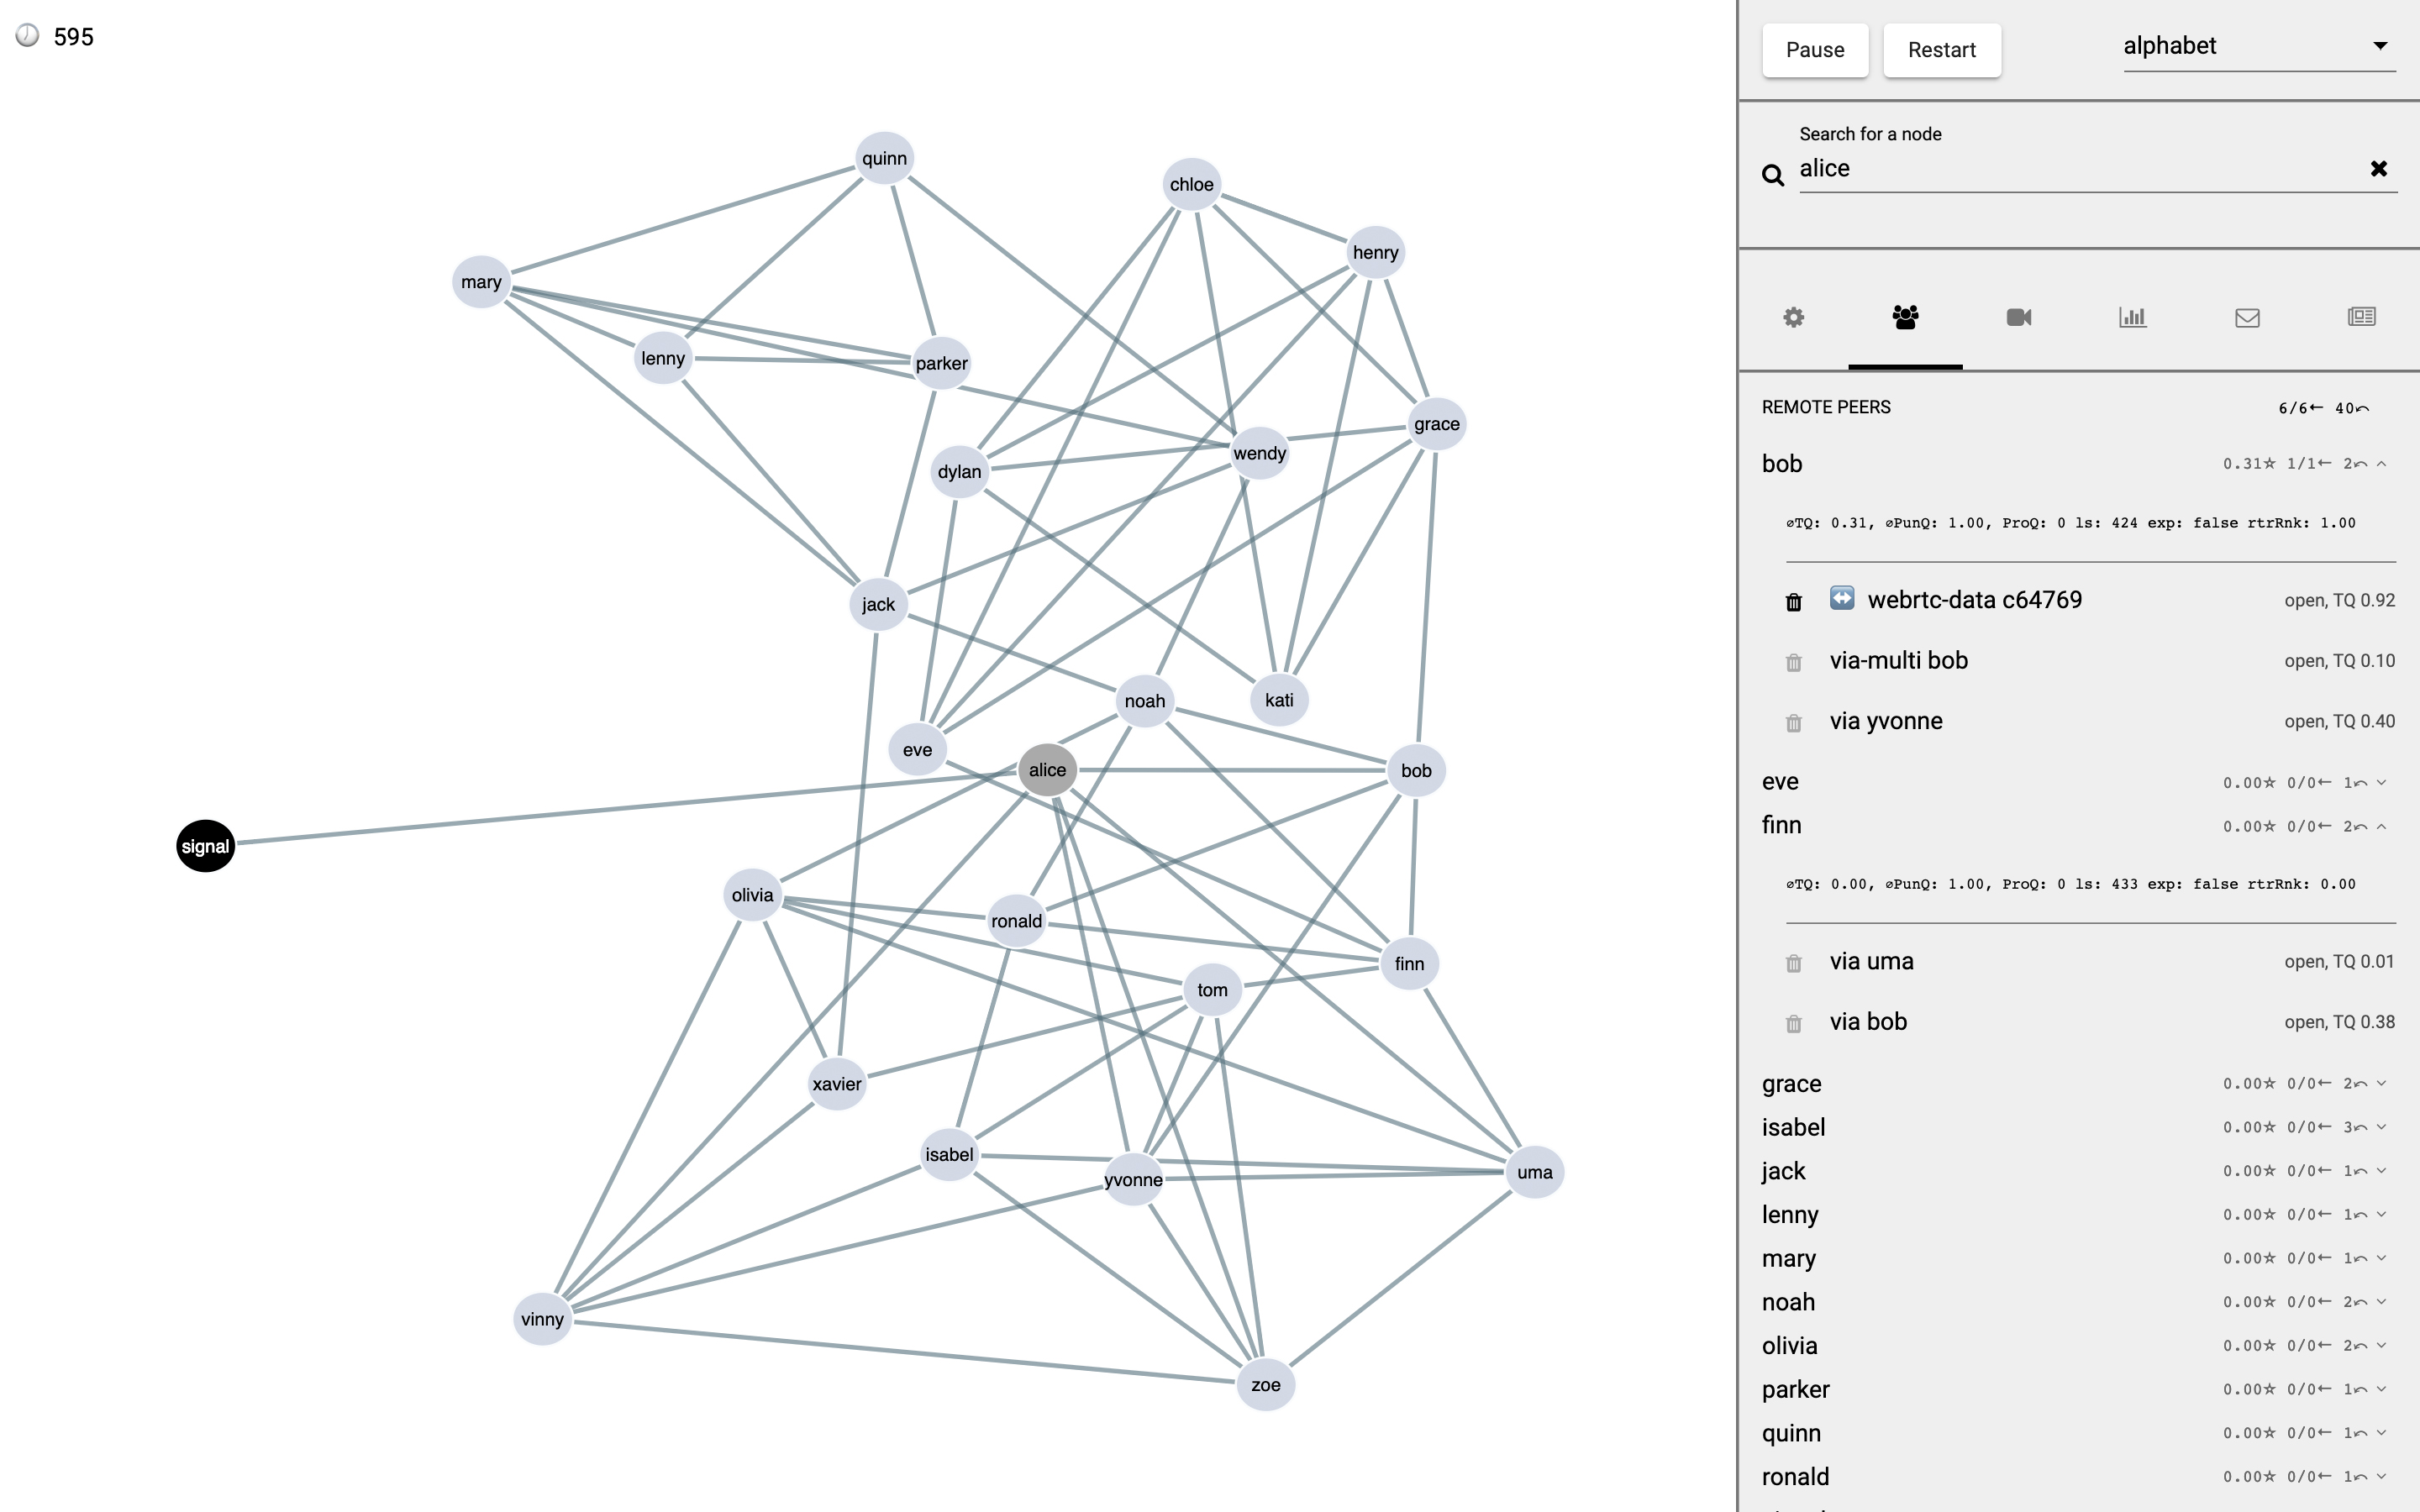
\includegraphics[width=1\textwidth]{graphics/analysis-tools/visualisation-overlay.jpg}
\caption{User interface of the Visualisation}
\label{fig:anl-visualisation}
\end{figure}

The Visualisation is build on top of the simulation and is presented in \vref{fig:anl-visualisation}. It takes the given output from the simulation and visualises its state. It is also using the global clock from the simulation and updates its state on every tick. Also it allows to interact with the nodes, like deleting it from the simulation or change the virtual network settings.

The interface consists of two parts. On the left side all nodes and their connections are represented as a graph. D3.js\footnote{D3.js. URL:{https://d3js.org/}} is used for the graph and further more the d3-force\footnote{D3.js d3-force module. URL:{https://github.com/d3/d3-force}} module is used.

Each node is represented as a circle with the node id as text label. Real names instead of pseudo ids were chosen for the node ids, to make it easier to discuss about a scenario. A node has also a colour which represents its role. Black represents a node with the role \signal. Dark grey a node with the role \router and light grey represents a node with the role \peer.  
When a node has a virtual connection to another node, the connection is represented as a grey line.
In the top left corner the current clock tick is displayed with an icon that indicates whether the clock is ticking or paused.

The sidebar on the right allows to interact with the simulation and to inspect a node. The first section allows to interact with the clock, pause, restart and a tick can be triggered. Also the scenario to execute can be chosen.

The section below allows to search for a node in the simulation. When a node for a search term was found it is automatically selected. A selected node is highlighted in the graph view but also the node inspection tool appears.

The inspection tool consists of six tabs and are presented in \vref{sec:visualisation-tabs}: 

Node settings, Peer table, Channel table, Network statistics, Incoming/Outgoing messages and Log entries. 

In the tab \textit{Channel table} a virtual stream can be started. The nodes behave like in the real world and broadcast their stream to other peers. The \glsfirst{dag} that is described in \vref{sec:design-stream-construction} is created. The visualisation is also able to visualise this graph as presented in \vref{fig:anl-sim-stream-active}. The black arrows indicate the direction of the stream from one node to another.

